\subsection*{Resultater}
Fra app'ens hovedmenu kan brugeren tilgå sine resultater, som visualiseres ved virtuelle belønninger.
Aktivitetsdiagrammet over resultater fremgår af \autoref{fig:resultater}.

\begin{figure} [H]
\centering
\textbf{Aktivitetsdiagram: Resultater}\par\medskip
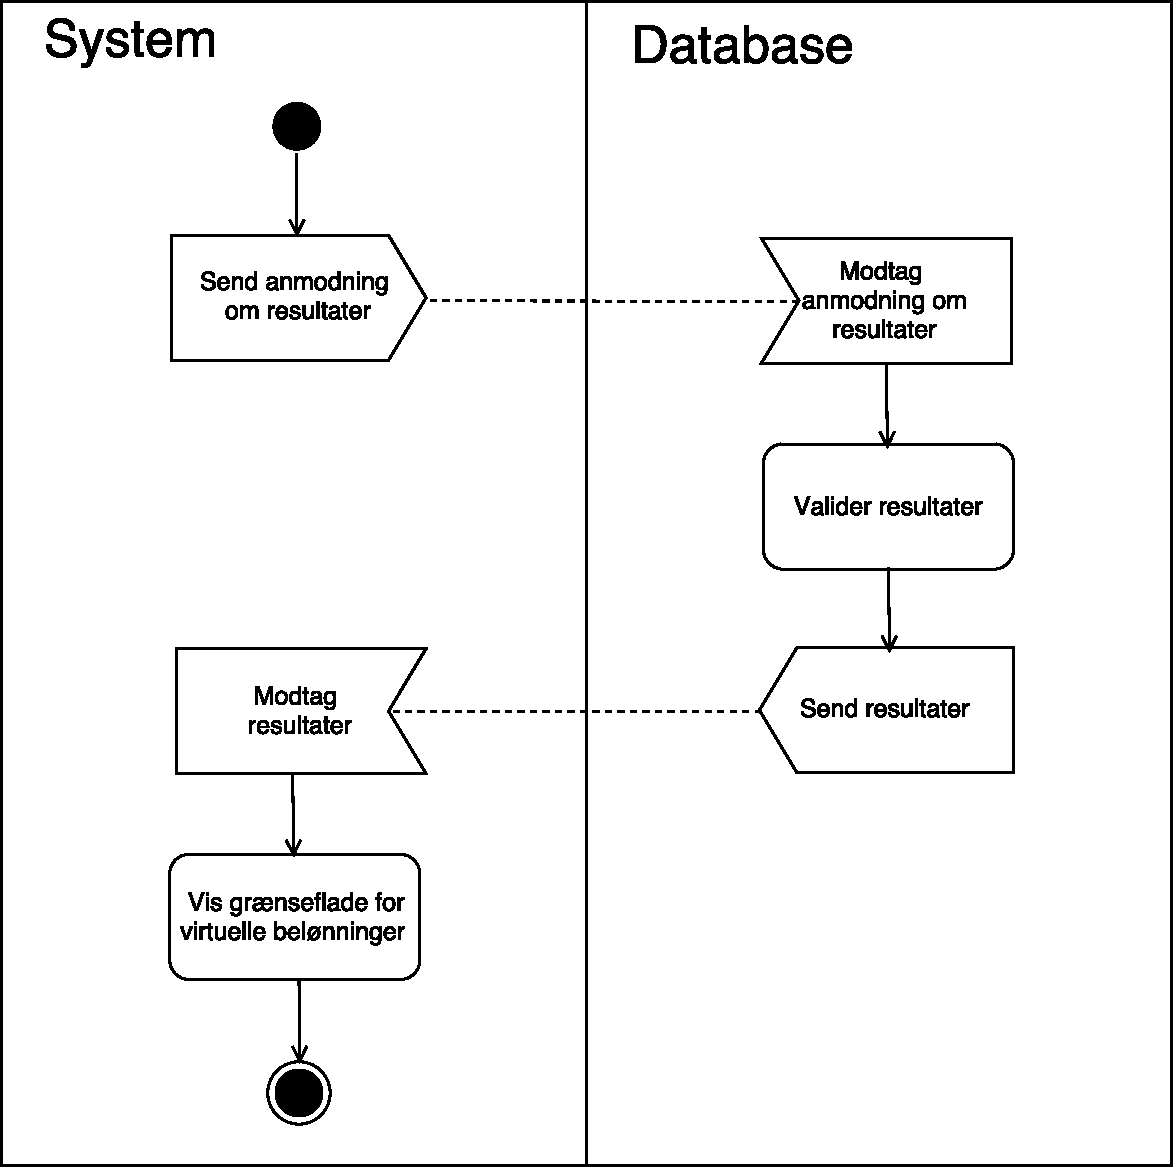
\includegraphics[width=0.9\textwidth]{figures/aktivitetsdiagram/Resultater}
\caption{Aktivitetsdiagram over resultater.}
\label{fig:resultater}
\end{figure}

\noindent
Under resultater er det muligt for brugeren at se sine virtuelle belønninger. Belønningerne varierer afhængig af træningsform og der kan opnås forskellige belønninger inden for forskellige kategorier. Et eksempel på fordeling af belønninger i forskellige kategorier fremgår af \autoref{tab:beloenninger}.

\begin{table} [H]
\centering
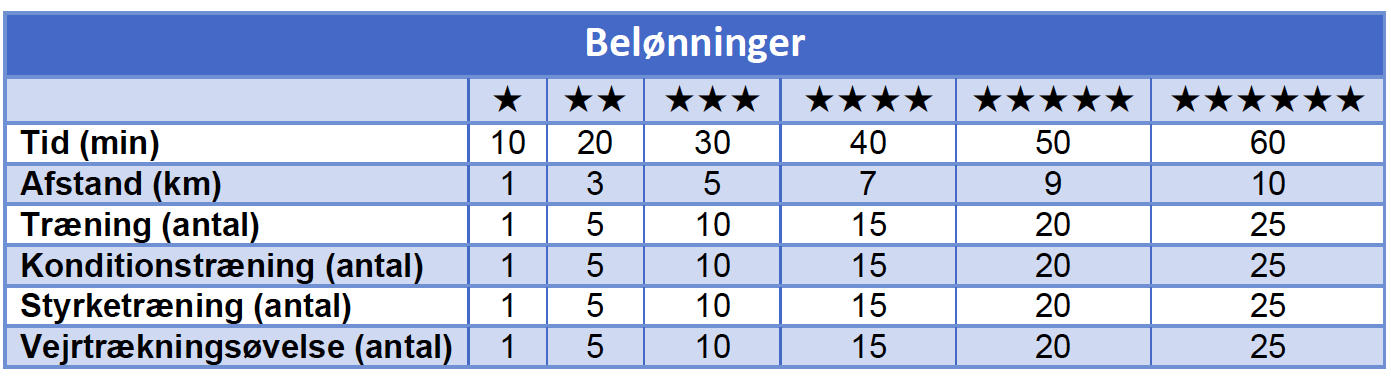
\includegraphics[width=1\textwidth]{figures/aktivitetsdiagram/beloenninger}
\caption{Eksempel på belønninger opnået ved træning inden for forskellige kategorier.}
\label{tab:beloenninger}
\end{table}

\noindent
Ud fra \autoref{tab:beloenninger} fremgår et eksempel på fordeling af virtuelle belønninger, der er opdelt efter afstand, tid og antallet af gennemførte træninger. 